%------------------- Bellows -------------------%
\subsection{Bellows} \label{subsec:bellows}

%------------------------------ Inputs and Outputs ------------------------------%
\subsubsection{Inputs and Outputs}
The bellow covering the hip and knee joints must be able to provide the required range of movement. The inputs include the available length for the bellow (nominal length), the required inner diameters of the conical bellow (chassis leg hole size and knee shaft size) and the required angular range of movement. The outputs are the number of folds required and their size. 

%------------------------------ CONSTANTS ------------------------------%
\subsubsection{Constants and Parameters}
The chosen minimum safety factor for the bellow is 2.5 as to stretch the bellow to its maximum or minimum on a regular basis could cause it to fail prematurely. The bellow may also bend or stretch in unpredictable ways, and is subjected to the movement of two joints. 
The thickness of the bellow is chosen to be a constant value of 3 mm for a balance of flexibility and sturdiness. The inner diameter depends on the required size of the hole in the chassis for the leg. The hip will be positioned as close as possible to the side of the chassis to ensure a smaller hole is required.

%------------------------------ Assumptions ------------------------------%
\subsubsection{Assumptions and Simplifications}
For the calculations, it is assumed that the bellow is bent into a circular bend. The safety factor is added to make up for any behavior deviating from this assumption. As the bellow covers two joints, it will sometimes be bending in two opposing directions. However, as the distance between the joints is small, these bends will likely cancel each other to a certain extent: the bellow might come to rest on the thigh member inside it, which is considered acceptable as no sharp edges will be present to wear out the bellow, and it will not interfere with any moving components. Thus, the analysis is carried out for the maximum total angle provided by both joints in the same direction.

As the bellow is conical, the required extension and retraction are calculated using the largest diameter of the bellow, as this gives the more stringent requirements.

%------------------------------ Materials ------------------------------%
\subsubsection{Material Selection}
The chosen material for the bellows is silicone as it is a moldable flexible material which is uv-resistant, waterproof and operates on a large range of temperatures \cite{custom_rubber_corp_rubber_nodate}.

%------------------------------ Free-Body Diagram ------------------------------%
\subsubsection{Free-Body Diagram}
The bellow analysis is mainly geometric, thus the required dimensions are shown in Figure \ref{fig:bellow}. The bellow at an angle is shown as being constant diameter, however the values with a conical bellow would be the same, but with using $d_{i,max}$ in calculations.

\begin{figure}
    \centering
    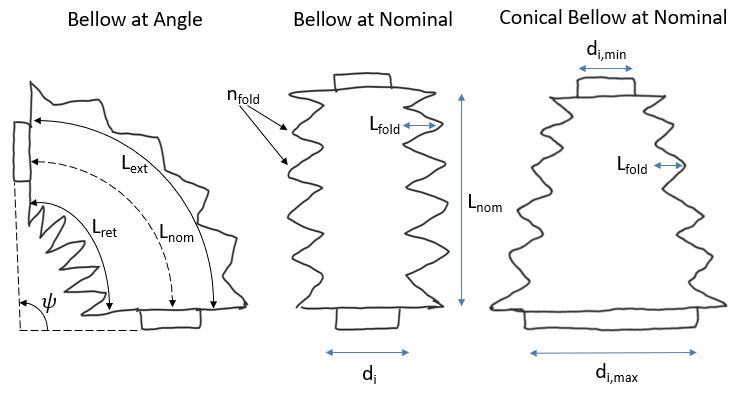
\includegraphics[width=\textwidth]{4_Analysis/img/Bellow/bellow.JPG}
    \caption{Bellow - Dimensions and Geometry}
    \label{fig:bellow}
\end{figure}

where $n_{fold}$ is the number of folds in the bellow, $L_{nom}$ is the nominal length of the bellow (straight un-extended), $L_{fold}$ is the height (or width) of the folds when the bellow is at nominal length, $d_i$ is the inner diameter of the bellow (max and min for conical bellow), $\psi$ is the bend angle of the bellow in degrees, $L_{ext}$ is the extended length of the bellow and $L_{ret}$ is the retracted length of the bellow.

To determine the required inner diameter of the bellow at the chassis, the following diagram is used:

\begin{figure}
    \centering
    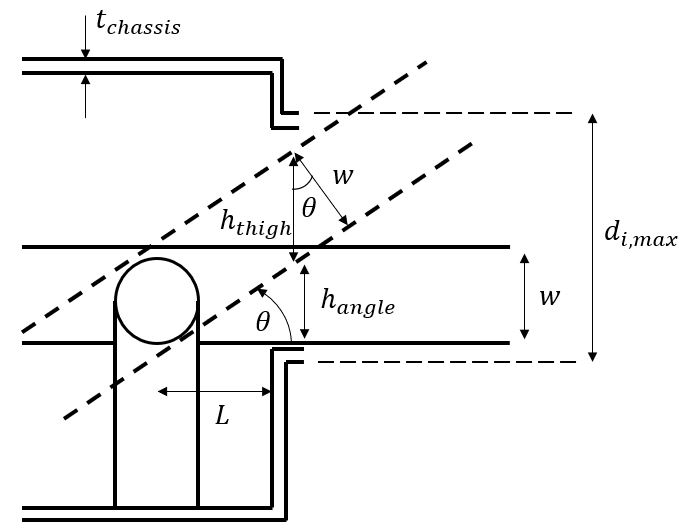
\includegraphics[width=0.7\textwidth]{4_Analysis/img/Bellow/bellowHole.JPG}
    \caption{Bellow - Finding the required inner diameter based on chassis leg hole}
    \label{fig:bellow_hole}
\end{figure}


%------------------------------ Geometrical Analysis ------------------------------%
\subsubsection{Analysis}
First, the required inner diameter of the bellow is computed using the following equation, based on Figure \ref{fig:bellow_hole}. We use $L=50mm$ based on harmonic drive diameter at the hip, $\theta=45^\circ$ the maximum angle of the hip, $w=70mm$ an approximation based on the pulley diameter and $t_{chassis}=5mm$.

\begin{equation}
    \begin{split}
       d_{i,max}=h_{angle}+h_{thigh}+2(t_{chassis})=L\tan{\theta}+\frac{w}{\cos{\theta}}+2t_{chassis}
       \\
       =50mm\tan{45^\circ}+\frac{70mm}{\cos{45^\circ}}+2(5mm)=159 mm \label{eq:bellow_hol} 
    \end{split}
\end{equation}

Next, the known geometrical values are used to find the required extended length and retracted length of the bellow. The nominal length and required angular range are used to get a nominal circumference $circ_{nom}$. The values used are $\psi=40.2^\circ$ the total angle of the hip and knee in the most extended position of the leg and $L_{nom}=94mm$ the approximated nominal length of the bellow based on limb lengths and space for the bellow hose clamps.

\begin{equation}
    circ_{nom}=\frac{360}{\psi}L_{nom}\frac{360}{40.2^\circ}94mm=841.5mm
\end{equation}

This value makes it easy to get the retracted and extended length by subtracting or adding an internal diameter (using the maximum value for the conical bellow) to get the inner and outer circumferences of the bend ($circ_i$ and $circ_o$) and converting back to lengths:

\begin{gather}
    circ_{o}=circ_{nom}+d_{i,max}=841.5 mm+159 mm=1000.5 mm
    \\
    L_{ext}=circ_{o}\div\frac{360}{\psi}=1000.5 mm \div\frac{360}{40.2^\circ}=111.8 mm
    \\
    circ_{i}=circ_{nom}-d_{i,max}=841.5mm-159 mm =682.5 mm
    \\
    L_{ret}=circ_{i}\div\frac{360}{\psi}=682.5 mm\div\frac{360}{40.2^\circ}=76.2 mm
\end{gather}

Now for the design of an appropriate bellow to fill those length requirements, the following expressions are used. The first finds the minimum retracted length $L_{min}$ of a bellow as a function of the number of folds $n_{fold}$ and the thickness of the bellow wall $t$. The second finds the maximum extended length $L_{max}$ of a bellow as a function of the number of folds and their "height" at nominal length $L_{fold}$. $t$ is a constant and is set to 3 mm and $n_{fold}$ and $L_{fold}$ are estimated until the proper safety factor is met.

\begin{gather}
    L_{min}=2n_{fold}t=2(8)(3mm)=48 mm \label{eq:bellow_min}
    \\
    L_{max}=2n_{fold}L_{fold}=2(8)(8.7 mm)=139.2 mm \label{eq:bellow_max}
\end{gather}

These values are then compared with the required values by calculating the extension/retraction value and finding the safety factor $SF$:

\begin{gather}
    SF=\frac{L_{max}-L_{nom}}{L_{ext}-L_{nom}}=\frac{139.2mm-94mm}{111.8mm-94mm}=2.5 \;\;Good! \label{eq:bellow_sf1}
    \\
    SF=\frac{L_{min}-L_{nom}}{L_{ret}-L_{nom}}=\frac{48mm-94mm}{76.2mm-94mm}=2.6 \;\;Good! \label{eq:bellow_sf2}
\end{gather}

Thus the bellow has 8 folds of 8.7 mm in size. The value of $d_{i,min}$ is chosen based on the length of the exterior knee shaft, plus some clearance, giving a value of about 102 mm.



%------------------------------ Critical Review ------------------------------%
\subsubsection{Critical Review}
The analysis (with the added safety factor) gives a reasonable estimate of the dimensions of the bellow. However it is difficult to know to which extent it is being over designed, as its behavior in movement is difficult to predict and the equations use approximations (such as the fact that the bellow bends in a perfectly circular shape).


%------------------------------ Parameterization ------------------------------%
\subsubsection{Parameterization}
The goal for the parameterization of this component is to use known geometry (nominal length, required angle, required inner diameters) to find an appropriate combination of the number of folds and their height at nominal length.